% =====================================================================
%  Cours simplifié pas à pas : modélisation et commande d'une chaîne
%  éolienne PMSG 2 MW (platitude + passivité + ANN)
%  Compilation : pdflatex cours_PMSG_fr.tex  (deux fois)
% =====================================================================
\pdfminorversion=4
\documentclass[11pt,a4paper]{article}
\usepackage[utf8]{inputenc}
\usepackage[T1]{fontenc}
\usepackage[french]{babel}
\usepackage{lmodern}
\usepackage[margin=2.2cm]{geometry}
\usepackage{amsmath,amssymb}
\usepackage{graphicx}
\usepackage{booktabs}
\usepackage{xcolor}
\usepackage[framemethod=default]{mdframed}
\usepackage[hidelinks]{hyperref}
\graphicspath{{figures/}}

\newcommand{\bv}[1]{\boldsymbol{#1}}
\definecolor{fondA}{RGB}{232,242,252}
\definecolor{fondB}{RGB}{255,244,229}
\definecolor{fondC}{RGB}{236,247,232}
\newmdenv[backgroundcolor=fondA,linecolor=blue!50!black,linewidth=0.8pt,innertopmargin=6pt,innerbottommargin=6pt]{idee}
\newmdenv[backgroundcolor=fondB,linecolor=orange!70!black,linewidth=0.8pt,innertopmargin=6pt,innerbottommargin=6pt]{exemple}
\newmdenv[backgroundcolor=fondC,linecolor=green!40!black,linewidth=0.8pt,innertopmargin=6pt,innerbottommargin=6pt]{resume}
\newcommand{\Idee}{\textbf{L'idée : }}
\newcommand{\Exemple}{\textbf{Exemple chiffré : }}
\newcommand{\Resume}{\textbf{À retenir : }}

\title{\textbf{Cours simplifié, pas à pas}\\[3mm]
\large Modélisation d'une chaîne éolienne à génératrice synchrone à aimants permanents (PMSG) de 2~MW\\
et sa commande par platitude + passivité + réseau de neurones (ANN)}
\author{Said Regani — Laboratoire L2EI, Université de Jijel}
\date{}

\begin{document}
\maketitle

\begin{idee}
\textbf{Comment lire ce document ?}
Il est écrit pour un étudiant qui ne connaît rien à la commande ni aux réseaux de neurones. On part de
zéro et on explique chaque équation : d'où elle vient, ce que signifie chaque terme, puis un exemple
avec les vrais chiffres de notre système.
Les encadrés bleus donnent \textbf{l'idée}, les orange un \textbf{exemple chiffré}, les verts ce
qu'il faut \textbf{retenir}.
\end{idee}

\tableofcontents
\newpage

% =====================================================================
\section{La vue d'ensemble : que fait le système ?}
% =====================================================================

Le système transforme \textbf{l'énergie du vent} en \textbf{électricité} injectée dans le réseau.
L'énergie traverse une chaîne d'éléments ; chacun la transforme d'une forme à une autre :

\begin{center}
\begin{tabular}{lll}
\toprule
Élément & Reçoit & Fournit\\
\midrule
Turbine & du vent & une rotation (couple $T_w$)\\
Génératrice (PMSG) & une rotation & un courant alternatif à fréquence variable\\
Redresseur MLI & du courant alternatif & du courant continu\\
Bus continu (bus DC) & du courant continu & stocke l'énergie un court instant (condensateur)\\
Onduleur MLI & du courant continu & du courant alternatif à 50~Hz\\
Filtre $L$ & un courant haché & un courant propre\\
Réseau 690~V & --- & reçoit l'énergie\\
\bottomrule
\end{tabular}
\end{center}

\paragraph{Pourquoi « back-to-back » ?}
Parce que le redresseur et l'onduleur sont reliés « dos à dos » par le bus continu. Cela découple la
génératrice du réseau : la génératrice tourne à vitesse variable (selon le vent) et le réseau reste
toujours à 50~Hz.

\paragraph{Pourquoi « attaque directe » ?}
La génératrice est montée directement sur l'arbre de la turbine, sans multiplicateur de vitesse.
Elle tourne donc lentement (environ 2~rad/s) et a besoin de beaucoup de pôles (26 paires).

\begin{figure}[h]
\centering
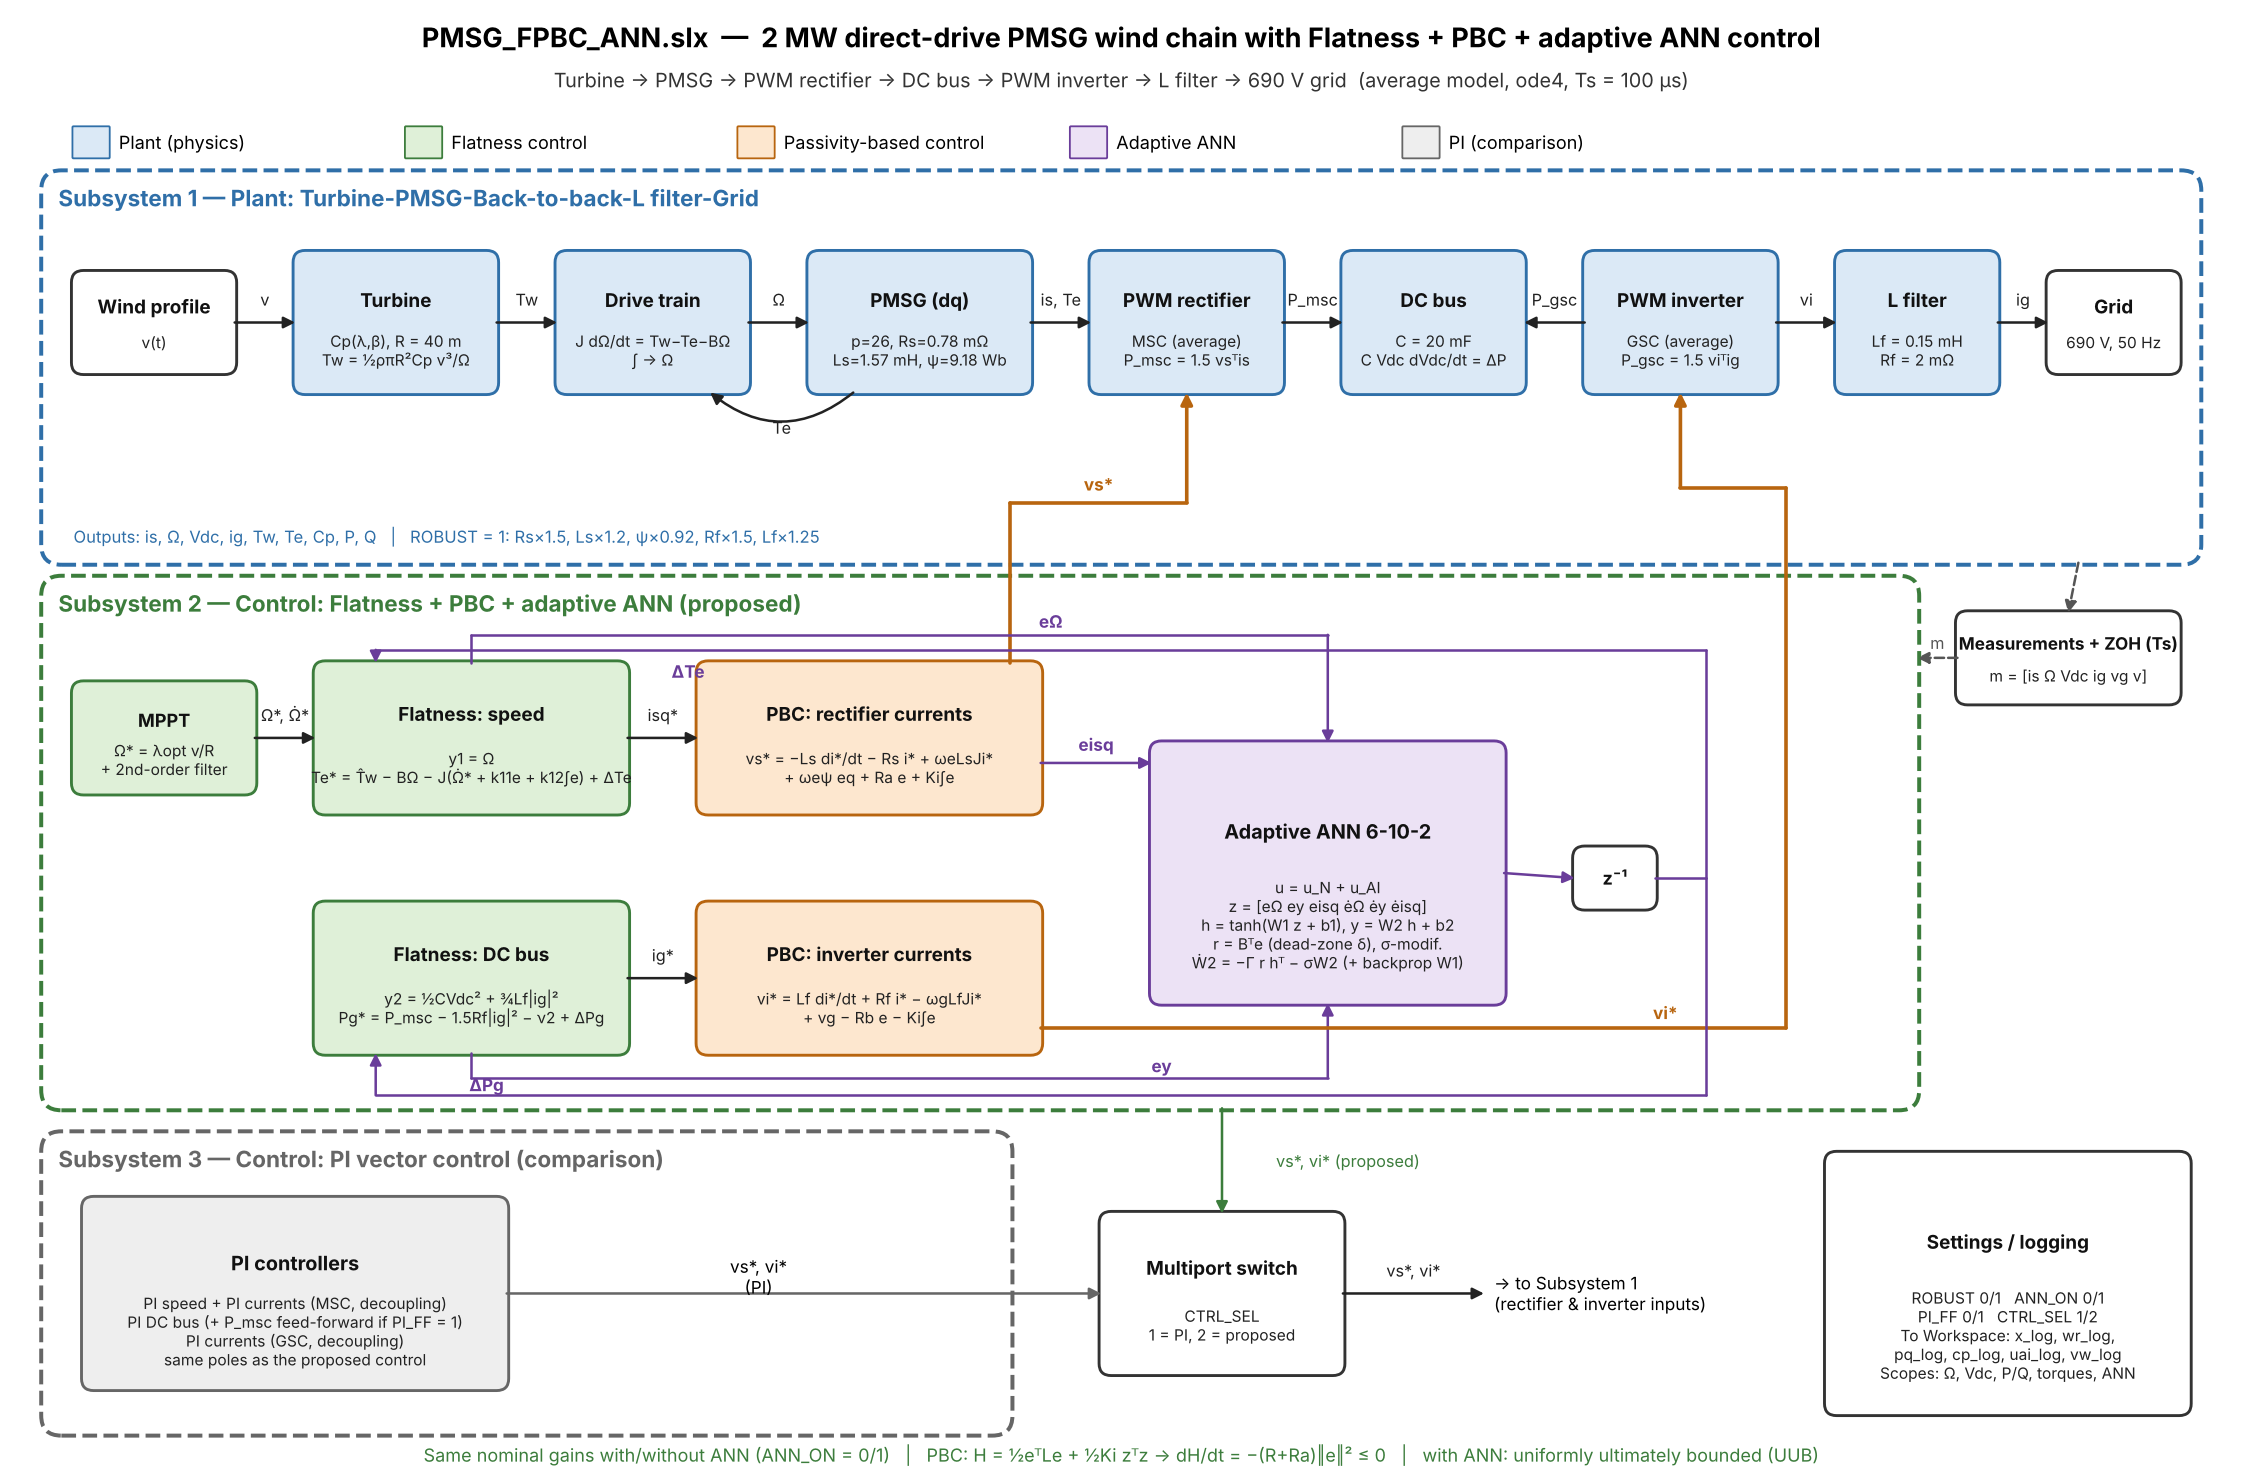
\includegraphics[width=\textwidth]{simulink_diagram.png}
\caption{Schéma complet : en haut le système physique, au milieu la commande.}
\end{figure}

\paragraph{Pourquoi a-t-on besoin d'une commande ?} Pour trois raisons :
\begin{enumerate}
\item \textbf{Extraire le maximum d'énergie} : pour chaque vitesse du vent il existe une vitesse de
rotation optimale. Il faut faire tourner la turbine à cette vitesse en permanence : c'est la \textbf{MPPT}.
\item \textbf{Garder la tension du bus continu constante} (1200~V) : trop haute, elle détruit les
condensateurs ; trop basse, l'onduleur ne peut plus produire la tension du réseau.
\item \textbf{Envoyer une énergie propre au réseau} : courant sinusoïdal et $Q=0$ (facteur de puissance 1).
\end{enumerate}

% =====================================================================
\section{La modélisation pas à pas}
% =====================================================================

\subsection{Qu'est-ce que modéliser ?}
\begin{idee}
\Idee
Modéliser, c'est écrire les \textbf{équations} qui décrivent comment chaque grandeur du système évolue
dans le temps. La plupart de nos équations ont la forme :
\[
\frac{d(\text{quelque chose})}{dt} = \text{ce qui entre} - \text{ce qui sort}.
\]
\textbf{Exemple du réservoir d'eau :} s'il entre 10~L/s et qu'il sort 7~L/s, le réservoir gagne 3~L
par seconde. C'est tout ! Toutes les équations du système reposent sur cette idée :
« variation = entrée $-$ sortie ».
\end{idee}

Le symbole $\frac{dx}{dt}$ (ou $\dot x$) signifie « vitesse de variation de $x$ ». S'il est positif,
$x$ augmente ; s'il est négatif, $x$ diminue ; s'il est nul, $x$ est constant (on dit que le système est
en \textbf{régime permanent}).

\subsection{Le vent}
On utilise la même équation du vent que dans notre article publié dans \emph{Mathematics} (équation 80) :
\begin{equation}
v(t) = V_{mean} + \sum_{k=1}^{3} A_k \sin(2\pi f_k t) + v_{turb}(t)
\end{equation}
\begin{itemize}
\item $V_{mean}=8$~m/s : la vitesse moyenne du vent.
\item $\sum A_k\sin(2\pi f_k t)$ : trois « vagues » lentes qui font monter et descendre le vent.
Valeurs : $A=[1{,}5;\ 0{,}2;\ 0{,}3]$~m/s et $f=[0{,}03;\ 0{,}16;\ 0{,}17]$~Hz.
\item $v_{turb}(t)$ : une petite perturbation aléatoire (environ $\pm 0{,}02$~m/s) qui représente les tourbillons.
\end{itemize}
Résultat : le vent part de 8, atteint 9 à $t=2$~s, redescend à 8,6, puis monte à 10~m/s vers $t=7{,}7$~s.

\subsection{La turbine : du vent au couple}

\paragraph{Étape 1 : combien d'énergie y a-t-il dans le vent ?}
Le vent est une masse d'air en mouvement : il a une énergie cinétique. La puissance qui traverse le
disque balayé par les pales (surface $\pi R^2$) vaut :
\begin{equation}
P_{vent} = \tfrac12\,\rho\,\pi R^2\, v^3
\end{equation}
avec $\rho=1{,}225$~kg/m$^3$ (masse volumique de l'air) et $R=40$~m (longueur de pale).
Remarque : la puissance est proportionnelle à $v^3$. Si le vent double, la puissance est multipliée par~\textbf{8} !

\paragraph{Étape 2 : quelle part la turbine récupère-t-elle ?}
La turbine ne peut pas tout récupérer (sinon l'air s'arrêterait derrière elle). La part récupérée est
le \textbf{coefficient de puissance} $C_p$ :
\begin{equation}
P_w = C_p(\lambda,\beta)\cdot \tfrac12\,\rho\,\pi R^2\, v^3
\end{equation}
En théorie, $C_p$ ne peut pas dépasser $0{,}593$ (limite de Betz). Pour notre turbine, le maximum est $0{,}48$.

\paragraph{Étape 3 : de quoi dépend $C_p$ ?}
De la \textbf{vitesse spécifique} :
\begin{equation}
\lambda = \frac{\Omega R}{v} = \frac{\text{vitesse du bout de pale}}{\text{vitesse du vent}}
\end{equation}
et de l'angle de calage des pales $\beta$ (pris égal à 0 car le vent reste inférieur au vent nominal).
La formule utilisée (modèle de Heier) :
\begin{equation}
C_p = 0{,}5176\left(\frac{116}{\lambda_i}-0{,}4\beta-5\right)e^{-21/\lambda_i}+0{,}0068\,\lambda,\qquad
\frac{1}{\lambda_i}=\frac{1}{\lambda+0{,}08\beta}-\frac{0{,}035}{\beta^3+1}
\end{equation}
Inutile de l'apprendre par c\oe ur : ce qui compte, c'est sa forme (figure~\ref{fig:cp}). Une seule
valeur $\lambda_{opt}=8{,}1$ donne le $C_p$ maximal.

\begin{figure}[h]
\centering
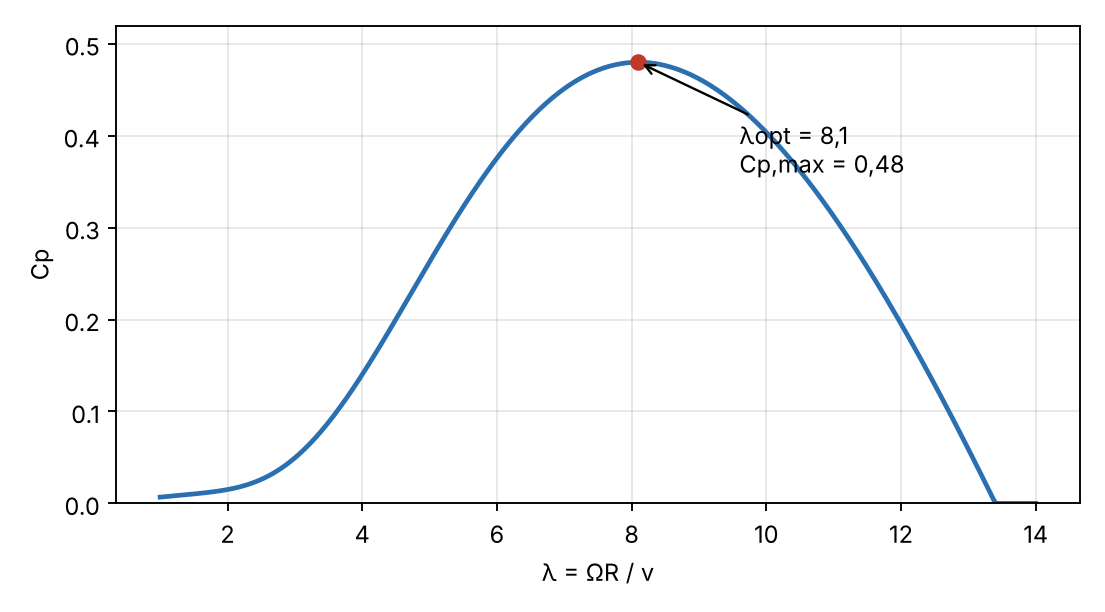
\includegraphics[width=0.62\textwidth]{cp_lambda.png}
\caption{Coefficient de puissance $C_p$ en fonction de $\lambda$ : un seul sommet en $\lambda_{opt}=8{,}1$.}
\label{fig:cp}
\end{figure}

\paragraph{Étape 4 : le couple aérodynamique.}
Puissance = couple $\times$ vitesse angulaire, donc :
\begin{equation}
T_w = \frac{P_w}{\Omega}
\end{equation}

\begin{exemple}
\Exemple
Vent $v=8$~m/s. Surface balayée : $\pi\times 40^2 = 5027$~m$^2$.
\begin{itemize}
\item Puissance dans le vent : $\tfrac12\times 1{,}225\times 5027\times 8^3 = 1{,}58$~MW.
\item Vitesse optimale : $\Omega = \lambda_{opt}\,v/R = 8{,}1\times 8/40 = 1{,}62$~rad/s (environ 15,5~tr/min).
\item Puissance récupérée : $0{,}48\times 1{,}58 = 0{,}76$~MW.
\item Couple : $T_w = 0{,}76\cdot 10^6/1{,}62 = 467$~kN$\cdot$m.
\end{itemize}
Au vent nominal ($\approx 11$~m/s) : $\Omega = 2{,}23$~rad/s et $P\approx 2$~MW, c'est bien la puissance
de la turbine. Les chiffres donnés par l'encadrant sont donc cohérents.
\end{exemple}

\subsection{L'arbre : du couple à la vitesse}
\begin{idee}
\Idee
C'est la loi de Newton pour la rotation. Le vent pousse (couple $T_w$), la génératrice « freine »
(couple $T_e$), et les frottements freinent un peu. Si la poussée est plus forte que le freinage, la
turbine accélère ; sinon, elle ralentit.
\end{idee}
\begin{equation}
J\,\frac{d\Omega}{dt} = T_w - T_e - B\,\Omega
\end{equation}
\begin{itemize}
\item $J=2{,}8\cdot10^6$~kg$\cdot$m$^2$ : l'inertie (plus elle est grande, plus il est difficile de changer la vitesse).
\item $T_e$ : le couple électromagnétique de la génératrice. \textbf{C'est lui que l'on commande !}
\item $B\Omega$ : les frottements ($B=1000$).
\end{itemize}

\begin{exemple}
\Exemple
Si $T_w - T_e = 100$~kN$\cdot$m, alors $\frac{d\Omega}{dt} = 10^5/(2{,}8\cdot 10^6) = 0{,}036$~rad/s$^2$.
Pour passer de 1,62 à 1,82~rad/s (quand le vent passe à 9~m/s), il faut environ 5,6~secondes.
La turbine est très lourde, donc lente.
\end{exemple}

\textbf{L'idée importante pour la commande :} pour faire tourner la turbine à la vitesse optimale,
on agit sur $T_e$ :
\begin{itemize}
\item si elle est trop lente, on \textbf{diminue} $T_e$ (on freine moins) et elle accélère ;
\item si elle est trop rapide, on \textbf{augmente} $T_e$ (on freine plus) et elle ralentit.
\end{itemize}

\subsection{La génératrice PMSG : de la rotation à l'électricité}

\paragraph{Étape 1 : comment produit-elle de l'électricité ?}
Le rotor porte des aimants permanents. Quand il tourne, le champ magnétique dans les bobines du stator
varie et fait apparaître une force électromotrice (f.é.m.) proportionnelle à la vitesse :
$E = \omega_e\,\psi_f$, où $\psi_f=9{,}18$~Wb est le flux des aimants.

\paragraph{Étape 2 : trois phases, puis la transformation de Park.}
La génératrice est triphasée : trois courants $i_a, i_b, i_c$ sinusoïdaux qui varient sans cesse.
Commander des grandeurs qui oscillent est difficile. On utilise donc la \textbf{transformation de Park} :
on décrit les courants du point de vue de quelqu'un qui tourne avec le rotor. Pour lui, les courants
n'oscillent plus : ils deviennent \textbf{deux grandeurs presque constantes} :
\begin{itemize}
\item $i_{sd}$ (axe $d$) : dans la direction des aimants. Il ne produit pas de couple.
\item $i_{sq}$ (axe $q$) : perpendiculaire aux aimants. C'est lui qui produit le couple.
\end{itemize}
\begin{idee}
\Idee
La transformation de Park, c'est comme monter sur un manège : les objets qui tournent avec vous
semblent immobiles. Les grandeurs alternatives deviennent ainsi « continues », et les commander devient facile.
\end{idee}

\paragraph{Étape 3 : les équations des tensions.}
Pour chaque axe, on écrit la loi de Kirchhoff : « tension produite dans la machine = tension perdue + tension de sortie ».
\begin{align}
L_s\frac{di_{sd}}{dt} &= \underbrace{-R_s i_{sd}}_{\text{perte résistive}}
\;+\;\underbrace{\omega_e L_s i_{sq}}_{\text{effet de l'autre axe}}
\;-\;\underbrace{v_{sd}}_{\text{tension du redresseur}}\\
L_s\frac{di_{sq}}{dt} &= -R_s i_{sq} - \omega_e L_s i_{sd}
\;+\;\underbrace{\omega_e\psi_f}_{\text{f.é.m. }E} \;-\; v_{sq}
\end{align}
\begin{itemize}
\item $R_s=0{,}78$~m$\Omega$ : résistance des bobines. $L_s=1{,}57$~mH : inductance (s'oppose à la variation du courant).
\item $\omega_e = p\,\Omega$ : vitesse électrique, avec $p=26$ paires de pôles.
\item $\omega_e L_s i$ : termes de \textbf{couplage} entre les deux axes, dus au fait que le repère tourne.
\item $v_{sd}, v_{sq}$ : la tension imposée par le redresseur. \textbf{C'est ce que l'on commande} pour piloter les courants.
\end{itemize}

\paragraph{Étape 4 : le couple.}
\begin{equation}
T_e = \tfrac32\, p\, \psi_f\, i_{sq}
\end{equation}
Le couple ne dépend que de $i_{sq}$. On choisit donc $i_{sd}^*=0$ (il ne sert à rien et crée des pertes)
et on règle le couple par $i_{sq}$.

\begin{exemple}
\Exemple
À $\Omega=1{,}62$~rad/s : $\omega_e = 26\times 1{,}62 = 42{,}1$~rad/s, soit une fréquence de 6,7~Hz
(et non 50 !). La f.é.m. vaut $E = 9{,}18\times 42{,}1 = 387$~V.
Pour produire $T_e = 467$~kN$\cdot$m il faut $i_{sq} = 467\,000/(1{,}5\times 26\times 9{,}18) = 1304$~A.
\end{exemple}

\paragraph{Étape 5 : écriture matricielle et une propriété très importante.}
On regroupe les deux équations : $\bv{i}_s=[i_{sd};\ i_{sq}]$, $\bv{v}_s=[v_{sd};\ v_{sq}]$ et
$\mathbf{J}=\begin{bmatrix}0&1\\-1&0\end{bmatrix}$ :
\begin{equation}
L_s\,\dot{\bv{i}}_s = -R_s\,\bv{i}_s + \omega_e L_s\,\mathbf{J}\,\bv{i}_s + \omega_e\psi_f\,\bv{e}_q - \bv{v}_s
\end{equation}
La matrice $\mathbf{J}$ est \textbf{antisymétrique} : $\bv{i}^T\mathbf{J}\,\bv{i} = i_d i_q - i_q i_d = 0$.
\begin{idee}
\Idee
Cela signifie que le terme de couplage $\omega_e L_s\mathbf{J}\bv{i}_s$ \textbf{ne produit ni ne consomme
d'énergie} : il la fait seulement passer d'un axe à l'autre (comme une force qui fait tourner un objet
sans l'accélérer). On dit qu'il est \textbf{« sans travail »}.
Cette propriété est la base de la commande passive, plus loin.
\end{idee}

\subsection{Les convertisseurs MLI : redresseur et onduleur}
\paragraph{Que fait la MLI (PWM) ?}
Le convertisseur est fait d'interrupteurs électroniques (IGBT) qui s'ouvrent et se ferment très vite
(2160 fois par seconde). En changeant la durée de fermeture (\textbf{rapport cyclique}), on fabrique une
tension « moyenne » de la valeur souhaitée.
\begin{idee}
\Idee
C'est comme une lampe qu'on allume et qu'on éteint très vite : si elle est allumée la moitié du temps,
on voit la moitié de la lumière.
\end{idee}

\paragraph{Le modèle moyen.}
On ne s'intéresse pas à chaque commutation, seulement à la valeur moyenne. On considère donc que le
convertisseur fournit directement la tension demandée, à condition de ne pas dépasser une limite :
\begin{equation}
\|\bv{v}\| \le \frac{V_{dc}}{\sqrt3} = \frac{1200}{1{,}732} = 693~\text{V}
\end{equation}
Le convertisseur ne perd pas d'énergie (hypothèse), donc puissance d'entrée = puissance de sortie :
\begin{equation}
P_{msc} = \tfrac32\,(v_{sd}i_{sd}+v_{sq}i_{sq}),\qquad P_{gsc} = \tfrac32\,(v_{id}i_{gd}+v_{iq}i_{gq})
\end{equation}

\subsection{Le bus continu : un réservoir d'énergie}
Le condensateur ($C=20$~mF) est comme un réservoir d'eau : le redresseur le remplit avec $P_{msc}$, l'onduleur
le vide avec $P_{gsc}$. L'énergie stockée vaut $W = \tfrac12 C V_{dc}^2$ et « variation = entrée $-$ sortie » :
\begin{equation}
\frac{dW}{dt} = P_{msc} - P_{gsc}\qquad\Longleftrightarrow\qquad C\,V_{dc}\frac{dV_{dc}}{dt}=P_{msc}-P_{gsc}
\end{equation}
\begin{exemple}
\Exemple
À 1200~V : $W = 0{,}5\times 0{,}02\times 1200^2 = 14{,}4$~kJ seulement.
S'il entre 100~kW de plus qu'il n'en sort, tout le stock change en $14{,}4/100 = 0{,}14$~s !
La commande de ce bus doit donc être \textbf{très rapide}.
\end{exemple}

\subsection{Le filtre $L$ et le réseau}
Le filtre est une bobine ($L_f=0{,}15$~mH, $R_f=2$~m$\Omega$) entre l'onduleur et le réseau. Il se comporte
exactement comme la PMSG, mais la « f.é.m. » est ici la tension du réseau $\bv{v}_g$ :
\begin{equation}
L_f\,\dot{\bv{i}}_g = -R_f\,\bv{i}_g + \omega_g L_f\,\mathbf{J}\,\bv{i}_g + \bv{v}_i - \bv{v}_g
\end{equation}
On oriente le repère de Park sur la tension du réseau (grâce à la PLL) : $v_{gd}=563$~V et $v_{gq}=0$. Alors :
\begin{equation}
P = \tfrac32\,v_{gd}\,i_{gd},\qquad Q = -\tfrac32\,v_{gd}\,i_{gq}
\end{equation}
Donc $i_{gd}$ règle la puissance active $P$ et $i_{gq}$ la puissance réactive $Q$ (on veut $Q=0$, donc $i_{gq}^*=0$).

\subsection{Le modèle complet : 6 variables}
\begin{resume}
\Resume
Tout le système est décrit par 6 \textbf{variables d'état}, chacune avec son équation :
\begin{center}
\begin{tabular}{lll}
\toprule
Variable & Signification & Équation qui la gouverne\\
\midrule
$i_{sd}, i_{sq}$ & courants de la génératrice & équations de la PMSG\\
$\Omega$ & vitesse de rotation & loi de Newton de l'arbre\\
$V_{dc}$ & tension du bus & bilan d'énergie du condensateur\\
$i_{gd}, i_{gq}$ & courants injectés au réseau & équations du filtre\\
\bottomrule
\end{tabular}
\end{center}
\textbf{Ce que l'on commande} (4 entrées) : $v_{sd}, v_{sq}$ (redresseur) et $v_{id}, v_{iq}$ (onduleur).\\
\textbf{Ce que l'on ne commande pas} (perturbations) : le vent $v$ et la tension du réseau $v_g$.
\end{resume}

\subsection{Les paramètres}
\begin{center}
\begin{tabular}{llll}
\toprule
Élément & Symbole & Valeur & Source\\
\midrule
Puissance nominale & $P_n$ & 2~MW & encadrant\\
Longueur de pale & $R$ & 40~m & encadrant\\
Vitesse nominale & $\Omega_n$ & 2,23~rad/s & encadrant\\
Couple nominal & $T_n$ & 0,9~MN$\cdot$m & encadrant\\
Paires de pôles & $p$ & 26 & article Hasan \& Shatil\\
Résistance statorique & $R_s$ & 0,78~m$\Omega$ & même article\\
Inductance & $L_s$ & 1,57~mH & même article\\
Flux des aimants & $\psi_f$ & 9,18~Wb & même article\\
Condensateur & $C$ & 20~mF & même article\\
Tension du bus & $V_{dc}^*$ & 1200~V & même article\\
Inductance du filtre & $L_f$ & 0,15~mH & même article\\
Inertie & $J$ & $2{,}8\cdot10^6$~kg$\cdot$m$^2$ & hypothèse\\
Réseau & & 690~V, 50~Hz & même article\\
\bottomrule
\end{tabular}
\end{center}

% =====================================================================
\section{La commande pas à pas}
% =====================================================================

\subsection{Qu'est-ce que commander ?}
\begin{idee}
\Idee
Exemple : vous voulez rouler à 80~km/h (c'est la \textbf{référence}). Vous regardez le compteur (la
\textbf{mesure}) et vous calculez l'écart (l'\textbf{erreur}) : si vous êtes à 70, l'erreur vaut $+10$,
donc vous appuyez sur l'accélérateur (la \textbf{commande}). C'est la \textbf{boucle fermée}.
Toute commande répond à une seule question : \textbf{de combien faut-il agir, en fonction de l'erreur ?}
\end{idee}

Dans la suite : $x^*$ est la référence (valeur désirée) et $e = x^* - x$ ou $e = x - x^*$ l'erreur.

\subsection{Pourquoi des boucles imbriquées (cascade) ?}
On a des grandeurs lentes (la vitesse : quelques secondes) et des grandeurs très rapides (les courants :
quelques millisecondes). On met donc deux niveaux de boucles :
\begin{itemize}
\item une \textbf{boucle externe lente}, qui décide « ce que l'on veut » (le couple ou la puissance désirés) ;
\item une \textbf{boucle interne rapide}, qui l'exécute en pilotant les courants.
\end{itemize}
\begin{figure}[h]
\centering
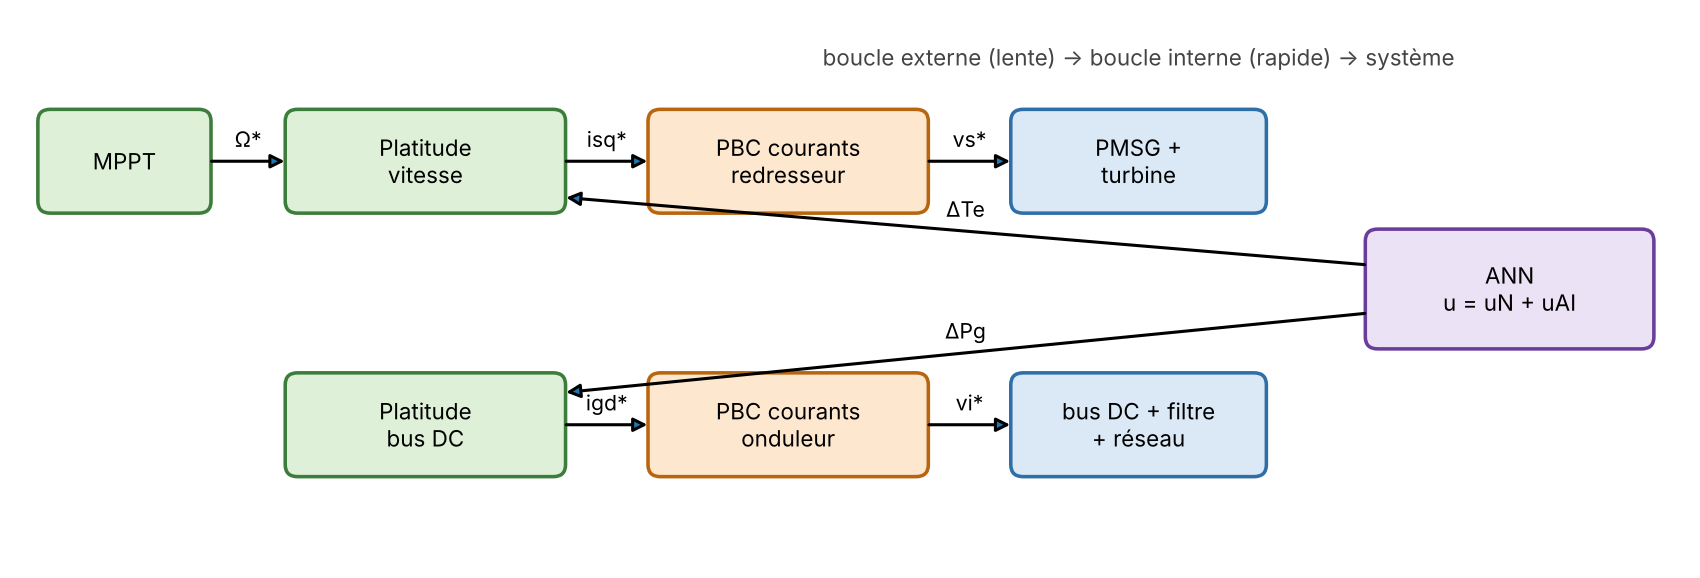
\includegraphics[width=\textwidth]{cascade.png}
\caption{Structure de la commande : en haut côté machine, en bas côté réseau, à droite le réseau de
neurones qui ajoute une correction.}
\end{figure}

\subsection{Étape 1 : la MPPT (où veut-on être ?)}
\begin{figure}[h]
\centering
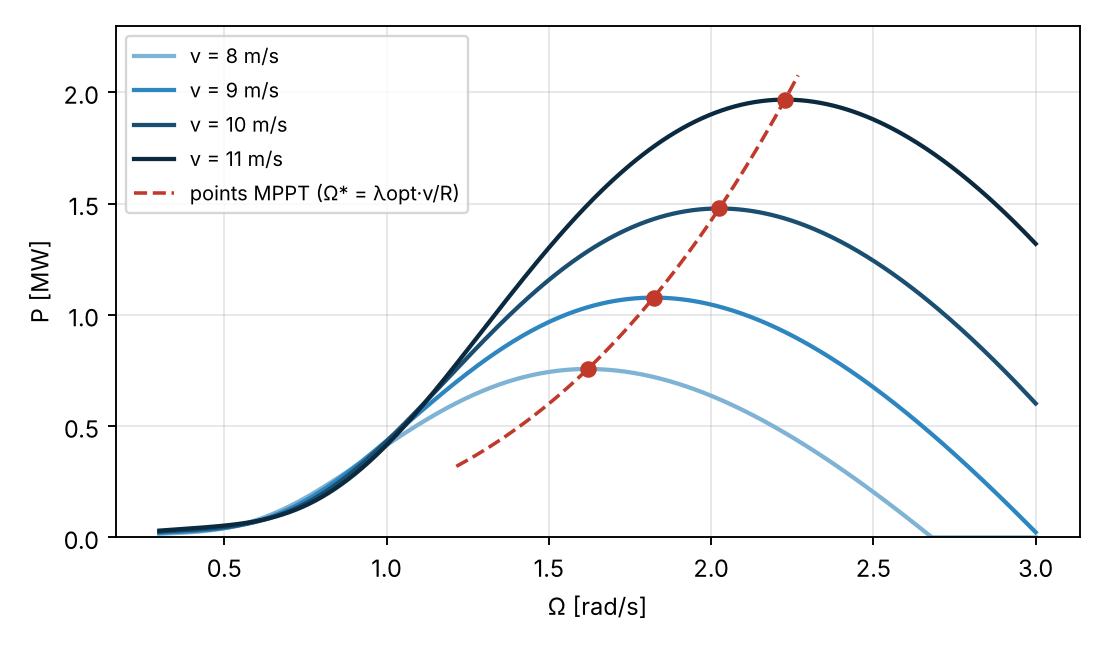
\includegraphics[width=0.62\textwidth]{mppt.png}
\caption{Puissance en fonction de la vitesse pour plusieurs vents. Les points rouges sont les sommets :
c'est là que l'on veut être.}
\end{figure}
Pour chaque vent, la puissance maximale est obtenue pour $\lambda=\lambda_{opt}$, c'est-à-dire :
\begin{equation}
\Omega^* = \frac{\lambda_{opt}\, v}{R}
\end{equation}
C'est la « vitesse de référence ». On la fait passer dans un filtre qui la rend lisse et qui donne
aussi sa dérivée $\dot\Omega^*$ (on en aura besoin).

\subsection{Rappel du régulateur PI (pour comprendre la suite)}
La commande la plus simple est le régulateur PI : $u = K_p\, e + K_i\int e\,dt$.
\begin{itemize}
\item La partie $K_p\,e$ (\textbf{proportionnelle}) : plus l'erreur est grande, plus la correction est forte.
\item La partie $K_i\int e$ (\textbf{intégrale}) : elle se souvient des erreurs passées et supprime la
petite erreur qui reste à la fin.
\end{itemize}
On retrouvera ces deux parties dans toutes nos lois (coefficients $k_{11}, k_{12}$, etc.). La différence :
nos lois utilisent en plus le \textbf{modèle physique}, ce qui les rend plus précises.

\subsection{Étape 2 : la commande par platitude}

\paragraph{L'idée en mots simples.}
\begin{idee}
\Idee
Au lieu d'attendre l'erreur pour corriger (comme un PI), on utilise l'équation physique
\textbf{à l'envers} : « je veux que la vitesse évolue comme ceci ; quel couple dois-je appliquer ? ».
L'équation donne directement la réponse. Puis on ajoute une petite correction (type PI) pour ce que le
modèle ignore.
On dit qu'un système est \textbf{plat} si l'on peut calculer tout (états et commandes) à partir d'une seule
« sortie » et de ses dérivées. Cette sortie s'appelle la \textbf{sortie plate}.
\end{idee}

\paragraph{La boucle de vitesse, pas à pas.}
\begin{enumerate}
\item On part de l'équation de l'arbre : $J\dot\Omega = T_w - T_e - B\Omega$.
\item On l'inverse pour calculer le couple : $T_e = T_w - B\Omega - J\dot\Omega$.
Si l'on connaît $\Omega$ et $\dot\Omega$, on connaît $T_e$ : la sortie plate est $y_1=\Omega$.
\item Que veut-on pour $\dot\Omega$ ? On veut que $\Omega$ suive $\Omega^*$. On choisit :
\[
\nu_1 = \underbrace{\dot\Omega^*}_{\text{suivre la référence}} + \underbrace{k_{11}\,e_\Omega}_{\text{corriger l'erreur}} + \underbrace{k_{12}\!\int\! e_\Omega}_{\text{supprimer l'erreur restante}},
\qquad e_\Omega = \Omega^* - \Omega
\]
\item On remplace $\dot\Omega$ par $\nu_1$, et $T_w$ (qu'on ne mesure pas) par sa valeur $\hat T_w$ calculée
avec l'équation de $C_p$ et le vent mesuré :
\begin{equation}
\boxed{T_e^* = \hat T_w - B\,\Omega - J\,\nu_1 + \Delta T_e}
\end{equation}
($\Delta T_e$ est la correction du réseau de neurones, expliquée plus loin.)
\item On convertit le couple en courant : $i_{sq}^* = T_e^*/(1{,}5\,p\,\psi_f)$ et $i_{sd}^*=0$.
\end{enumerate}
\textbf{Pourquoi ça marche ?} Si $\hat T_w = T_w$ exactement, en remplaçant dans l'équation de l'arbre on trouve :
\[
\dot e_\Omega + k_{11}\,e_\Omega + k_{12}\!\int\! e_\Omega = 0 .
\]
C'est l'équation d'une erreur qui « s'éteint » d'elle-même (comme un ressort avec un amortisseur). On choisit
$k_{11}=2\zeta\omega_n=3{,}6$ et $k_{12}=\omega_n^2=4$ (avec $\omega_n = 2$~rad/s et $\zeta=0{,}9$) : l'erreur
disparaît en environ deux secondes sans grosse oscillation.

\paragraph{La boucle du bus continu, pas à pas.}
\begin{enumerate}
\item La sortie plate est ici \textbf{l'énergie stockée} (dans le condensateur et dans les bobines du filtre) :
$y_2 = \tfrac12 C V_{dc}^2 + \tfrac34 L_f\|\bv{i}_g\|^2$.
\item Pourquoi l'énergie et pas la tension ? Parce que l'équation de l'énergie est \textbf{linéaire et simple},
« variation = entrée $-$ sortie » :
\[
\dot y_2 = P_{msc} - \underbrace{\tfrac32 v_{gd} i_{gd}}_{P_g\ \text{(vers le réseau)}} - \underbrace{\tfrac32 R_f\|\bv{i}_g\|^2}_{\text{pertes du filtre}}
\]
\item On l'inverse : pour avoir $\dot y_2 = -\nu_2$, il faut envoyer au réseau :
\begin{equation}
\boxed{P_g^* = P_{msc} - \tfrac32 R_f\|\bv{i}_g\|^2 - \nu_2 + \Delta P_g},\qquad
\nu_2 = k_{21}\,e_y + k_{22}\!\int\! e_y,\quad e_y = y_2^*-y_2
\end{equation}
\item En mots : « envoie au réseau tout ce qui vient de la génératrice ($P_{msc}$), moins les pertes, et
corrige un peu si l'énergie stockée s'éloigne de sa référence ».
\item On convertit la puissance en courant : $i_{gd}^* = 2P_g^*/(3 v_{gd})$ et $i_{gq}^* = 0$.
\end{enumerate}
\textbf{Pourquoi est-ce bien ?} Parce que la loi \textbf{anticipe} : dès que $P_{msc}$ change, $P_g^*$ change
immédiatement, avant que la tension ne bouge. C'est pourquoi $V_{dc}$ reste presque constant ($\pm 0{,}4$~V).

\subsection{Étape 3 : la commande passive (PBC) des courants}

\paragraph{L'idée en mots simples.}
\begin{idee}
\Idee
Un système \textbf{passif} ne crée pas d'énergie à partir de rien : son énergie stockée ne peut augmenter que
si on lui en fournit de l'extérieur. Comme une bille dans un bol : si on la lâche, elle roule puis s'arrête
au fond grâce au frottement.\\
La commande passive dit : \textbf{faire en sorte que « l'énergie de l'erreur » se comporte comme cette bille.}
On écrit une énergie pour l'erreur et on conçoit la commande pour que cette énergie diminue toujours.
L'erreur va alors forcément vers zéro.
\end{idee}

\paragraph{Pas à pas (pour le redresseur).}
\begin{enumerate}
\item On définit l'erreur : $\bv{e}_s = \bv{i}_s - \bv{i}_s^*$.
\item On veut que l'erreur ait la même forme que l'équation de la PMSG, avec un \textbf{frottement
supplémentaire} $R_a$ (\textbf{injection d'amortissement}, comme l'amortisseur d'une voiture) et une partie
intégrale $K_i$ :
\[
L_s\dot{\bv{e}}_s = -(R_s+R_a)\,\bv{e}_s + \omega_e L_s\,\mathbf{J}\,\bv{e}_s - K_i\!\int\!\bv{e}_s
\]
\item Pour obtenir cela, on calcule la tension que doit appliquer le redresseur (on remplace dans
l'équation de la PMSG et on résout) :
\begin{equation}
\boxed{\bv{v}_s^* = -L_s\dot{\bv{i}}_s^* - R_s\bv{i}_s^* + \omega_e L_s\mathbf{J}\,\bv{i}_s^* + \omega_e\psi_f\,\bv{e}_q + R_a\,\bv{e}_s + K_i\!\int\!\bv{e}_s}
\end{equation}
Terme par terme :
\begin{itemize}
\item $-L_s\dot{\bv{i}}_s^* - R_s\bv{i}_s^*$ : la tension « théorique » pour que le courant suive sa référence.
\item $\omega_e L_s\mathbf{J}\bv{i}_s^*$ : on garde le couplage (puisqu'il est sans travail), mais calculé sur la référence.
\item $\omega_e\psi_f\bv{e}_q$ : on compense la f.é.m. de la génératrice.
\item $R_a\bv{e}_s$ : le frottement supplémentaire qui « tue » l'erreur.
\item $K_i\int\bv{e}_s$ : supprime la petite erreur restante (si les paramètres ne sont pas exacts).
\end{itemize}
\end{enumerate}

\paragraph{Pourquoi est-ce stable ? (la preuve en mots)}
On prend « l'énergie de l'erreur » :
\[
H = \underbrace{\tfrac12 L_s\|\bv{e}_s\|^2}_{\text{énergie magnétique de l'erreur}} + \underbrace{\tfrac12 K_i\|\textstyle\int\bv{e}_s\|^2}_{\text{énergie de l'intégrale}}
\]
On calcule sa variation et on trouve :
\[
\frac{dH}{dt} = -(R_s+R_a)\,\|\bv{e}_s\|^2 \;+\; \underbrace{\omega_e L_s\,\bv{e}_s^T\mathbf{J}\,\bv{e}_s}_{=0\ \text{(sans travail !)}} \;=\; -(R_s+R_a)\,\|\bv{e}_s\|^2 \le 0 .
\]
\begin{resume}
\Resume
L'énergie de l'erreur \textbf{n'augmente jamais} et diminue tant qu'il reste une erreur : l'erreur va donc
vers zéro. On a utilisé la propriété « sans travail » de $\mathbf{J}$ : le terme de couplage a disparu du calcul.
C'est le c\oe ur de la commande passive : \textbf{respecter la structure énergétique du système au lieu de la combattre}.
\end{resume}

Même chose pour l'onduleur et le filtre :
\begin{equation}
\boxed{\bv{v}_i^* = L_f\dot{\bv{i}}_g^* + R_f\bv{i}_g^* - \omega_g L_f\mathbf{J}\,\bv{i}_g^* + \bv{v}_g - R_b\,\bv{e}_g - K_{ig}\!\int\!\bv{e}_g}
\end{equation}

\paragraph{Les valeurs.} On choisit une constante de temps $\tau_i = 2$~ms (les courants sont très rapides) :
$R_a = L_s/\tau_i = 0{,}785~\Omega$ et $R_b = L_f/\tau_i = 0{,}075~\Omega$.

\subsection{Qu'est-ce qu'une fonction de Lyapunov ?}
\begin{idee}
\Idee
Une fonction de Lyapunov est une « énergie » que l'on invente pour l'erreur : elle est toujours positive et
ne vaut zéro que si l'erreur est nulle. Si l'on prouve qu'elle \textbf{diminue toujours} avec le temps,
l'erreur est obligée d'aller vers zéro, comme une bille qui descend au fond d'un bol. La fonction $H$
utilisée plus haut est une fonction de Lyapunov.
\end{idee}

% =====================================================================
\section{Le réseau de neurones (ANN) pas à pas}
% =====================================================================

\subsection{Pourquoi en a-t-on besoin ?}
La loi de platitude utilise $\hat T_w$, calculé avec l'équation de $C_p$. Mais en réalité, l'équation de
$C_p$ n'est \textbf{jamais exacte} (pales encrassées, masse volumique de l'air qui change, etc.). Dans le
test de robustesse, on a rendu $\hat T_w$ 10\,\% plus petit que la réalité. Résultat : il reste une petite
erreur de vitesse qui ne disparaît pas vite.
\begin{idee}
\Idee
Le réseau de neurones « apprend » cette erreur pendant le fonctionnement et la corrige. Il \textbf{ne remplace
pas} la commande de base : il \textbf{ajoute} une petite correction :
\[
u = \underbrace{u_N}_{\text{commande de base}} + \underbrace{u_{AI}}_{\text{correction du réseau}},
\qquad u_{AI} = [\Delta T_e;\ \Delta P_g]
\]
et il ne modifie pas les coefficients de la commande de base ($k_{11}$, $R_a$, etc.). C'est la même méthode
que dans notre article de \emph{Mathematics}.
\end{idee}

\subsection{Le neurone seul}
Un neurone est un calcul très simple :
\begin{enumerate}
\item il reçoit plusieurs entrées $z_1, z_2, \dots$ ;
\item il multiplie chaque entrée par un \textbf{poids} $w_1, w_2, \dots$, fait la somme et ajoute un
\textbf{biais} $b$ : $a = w_1 z_1 + w_2 z_2 + \dots + b$ ;
\item il fait passer le résultat dans une \textbf{fonction d'activation}. On utilise $\tanh$, qui a la forme
d'un S et donne une valeur entre $-1$ et $+1$.
\end{enumerate}
\begin{exemple}
\Exemple
Deux entrées $z=[0{,}5;\ -0{,}2]$, des poids $w=[0{,}8;\ 0{,}3]$ et $b=0{,}1$ :\\
$a = 0{,}8\times 0{,}5 + 0{,}3\times(-0{,}2) + 0{,}1 = 0{,}44$, et la sortie vaut $h = \tanh(0{,}44) = 0{,}41$.
\end{exemple}
\textbf{Les poids sont la « mémoire » du réseau.} Apprendre, c'est modifier les poids.

\subsection{Le réseau 6-10-2}
\begin{figure}[h]
\centering
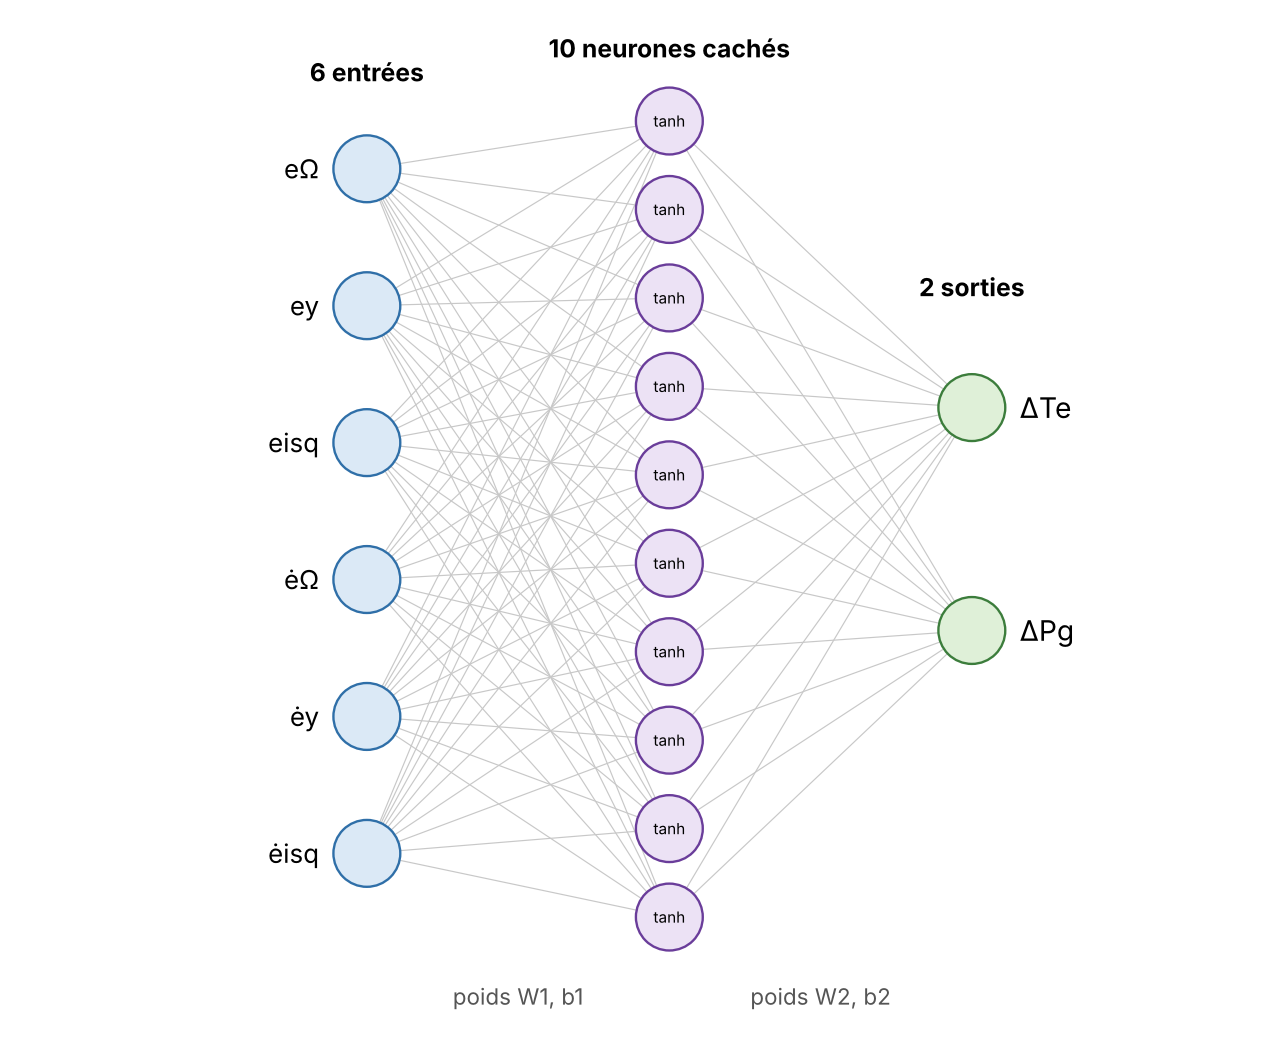
\includegraphics[width=0.6\textwidth]{ann.png}
\caption{Le réseau de neurones : 6 entrées, 10 neurones cachés, 2 sorties.}
\end{figure}
\begin{itemize}
\item \textbf{6 entrées} : les trois erreurs et leurs dérivées :
$e_\Omega$ (erreur de vitesse), $e_y$ (erreur d'énergie du bus), $e_{isq}$ (erreur de courant), et
$\dot e_\Omega, \dot e_y, \dot e_{isq}$. On les divise par des valeurs de référence (\textbf{normalisation})
pour qu'elles soient toutes de la même taille (autour de 1).
\item \textbf{10 neurones cachés} (couche cachée) : chacun calcule $h_j = \tanh(\sum_i W_{1,ji} z_i + b_{1,j})$.
En matrices : $\bv{h} = \tanh(W_1\bv{z} + \bv{b}_1)$, où $W_1$ est une matrice $10\times 6$ (60 poids).
\item \textbf{2 sorties} : $\bv{y} = W_2\bv{h} + \bv{b}_2$, où $W_2$ est une matrice $2\times 10$.
Les sorties sont $\Delta T_e$ et $\Delta P_g$ (après multiplication par les échelles $0{,}1\,T_n$ et $0{,}1\,P_n$).
\end{itemize}

\subsection{Comment apprend-il ? (la partie la plus importante)}

\paragraph{Étape 1 : que veut-on réduire ?} L'erreur. Si l'erreur est nulle, il n'y a rien à apprendre.

\paragraph{Étape 2 : dans quel sens corriger ?}
On raisonne avec la physique : si $e_\Omega = \Omega^*-\Omega > 0$, la turbine est \textbf{trop lente}.
Pour qu'elle accélère, il faut \textbf{diminuer} le couple de freinage $T_e$, donc $\Delta T_e$ doit diminuer.
Même logique pour le bus : si $e_y>0$ (énergie insuffisante), il faut envoyer moins au réseau, donc $\Delta P_g$ diminue.
\begin{idee}
\Idee
On appelle \textbf{signal d'apprentissage} $\bv{r} = [e_\Omega;\ e_y]$ (dans l'article : $\bv{r}=B^T\bv{e}$,
c'est-à-dire l'erreur dans la direction de la commande).
La règle : \textbf{déplacer la sortie dans le sens opposé au signal d'apprentissage.}
\end{idee}

\paragraph{Étape 3 : corriger les poids de sortie.}
\begin{equation}
\dot W_2 = -\Gamma\,\bv{r}\,\bv{h}^T - \sigma W_2
\end{equation}
\begin{itemize}
\item $-\Gamma\,\bv{r}\,\bv{h}^T$ : on change chaque poids proportionnellement à l'erreur ($\bv{r}$) multipliée
par l'activité du neurone relié ($\bv{h}$). Un neurone actif porte plus de « responsabilité », donc son poids change plus.
\item $\Gamma=5$ : la vitesse d'apprentissage (gain d'adaptation).
\item $-\sigma W_2$ (avec $\sigma=0{,}01$) : un petit « oubli » qui empêche les poids d'exploser ($\sigma$-modification).
\end{itemize}
\begin{exemple}
\Exemple
Supposons la turbine un peu trop lente : $e_\Omega = 0{,}5$ (après normalisation), $e_y=0$, et le premier
neurone a une activité $h_1 = 0{,}4$. La variation du poids $W_{2,11}$ (qui relie le neurone 1 à $\Delta T_e$) :
\[
\dot W_{2,11} = -5\times 0{,}5\times 0{,}4 = -1\ \text{par seconde}.
\]
En un pas ($T_s = 0{,}0001$~s), le poids change de $-0{,}0001$. Après des milliers de pas, $\Delta T_e$
diminue nettement, la turbine accélère et l'erreur diminue. \textbf{C'est cela, apprendre.}
\end{exemple}

\paragraph{Étape 4 : corriger les poids de la couche cachée (rétropropagation).}
On répartit la « responsabilité » de la sortie vers les neurones cachés :
\begin{equation}
\bv{\delta}_h = (1-\bv{h}^2)\odot(W_2^T\bv{r}),\qquad \dot W_1 = -\Gamma\,\bv{\delta}_h\,\bv{z}^T - \sigma W_1
\end{equation}
\begin{itemize}
\item $W_2^T\bv{r}$ : la contribution de chaque neurone caché à l'erreur (selon son poids vers la sortie).
\item $(1-\bv{h}^2)$ : la dérivée de $\tanh$. Un neurone « saturé » (proche de $\pm1$) apprend moins.
\item $\odot$ : multiplication élément par élément.
\end{itemize}

\paragraph{Étape 5 : les précautions.}
\begin{itemize}
\item \textbf{Zone morte} ($\delta = 0{,}1$) : si l'erreur est très petite, on n'apprend pas. Cela évite
d'« apprendre le bruit ».
\item \textbf{Saturation} : la sortie est limitée à $\pm 0{,}3\,T_n$ et $\pm 0{,}3\,P_n$, pour éviter une correction dangereuse.
\item \textbf{Gel} : si le couple ou le courant est à sa limite, on arrête l'apprentissage.
\item \textbf{Retard} : la sortie calculée maintenant est utilisée au pas suivant.
\end{itemize}

\subsection{Est-ce sûr ? (la stabilité)}
\begin{idee}
\Idee
La commande de base est stable (on l'a prouvé avec une fonction de Lyapunov). Le réseau ajoute quelque chose
de petit et borné, et ses poids n'explosent pas grâce à $\sigma$. Résultat (même théorème 2 que dans l'article
\emph{Mathematics}) : l'erreur reste \textbf{bornée dans une petite zone autour de zéro}. On dit qu'elle est
\textbf{uniformément ultimement bornée (UUB)}.\\
\textbf{Attention :} si l'apprentissage est trop rapide ($\Gamma\ge 20$), la boucle du bus devient instable en
simulation. C'est pourquoi on a choisi $\Gamma = 5$.
\end{idee}

\subsection{Qu'a réellement appris le réseau ?}
\begin{figure}[h]
\centering
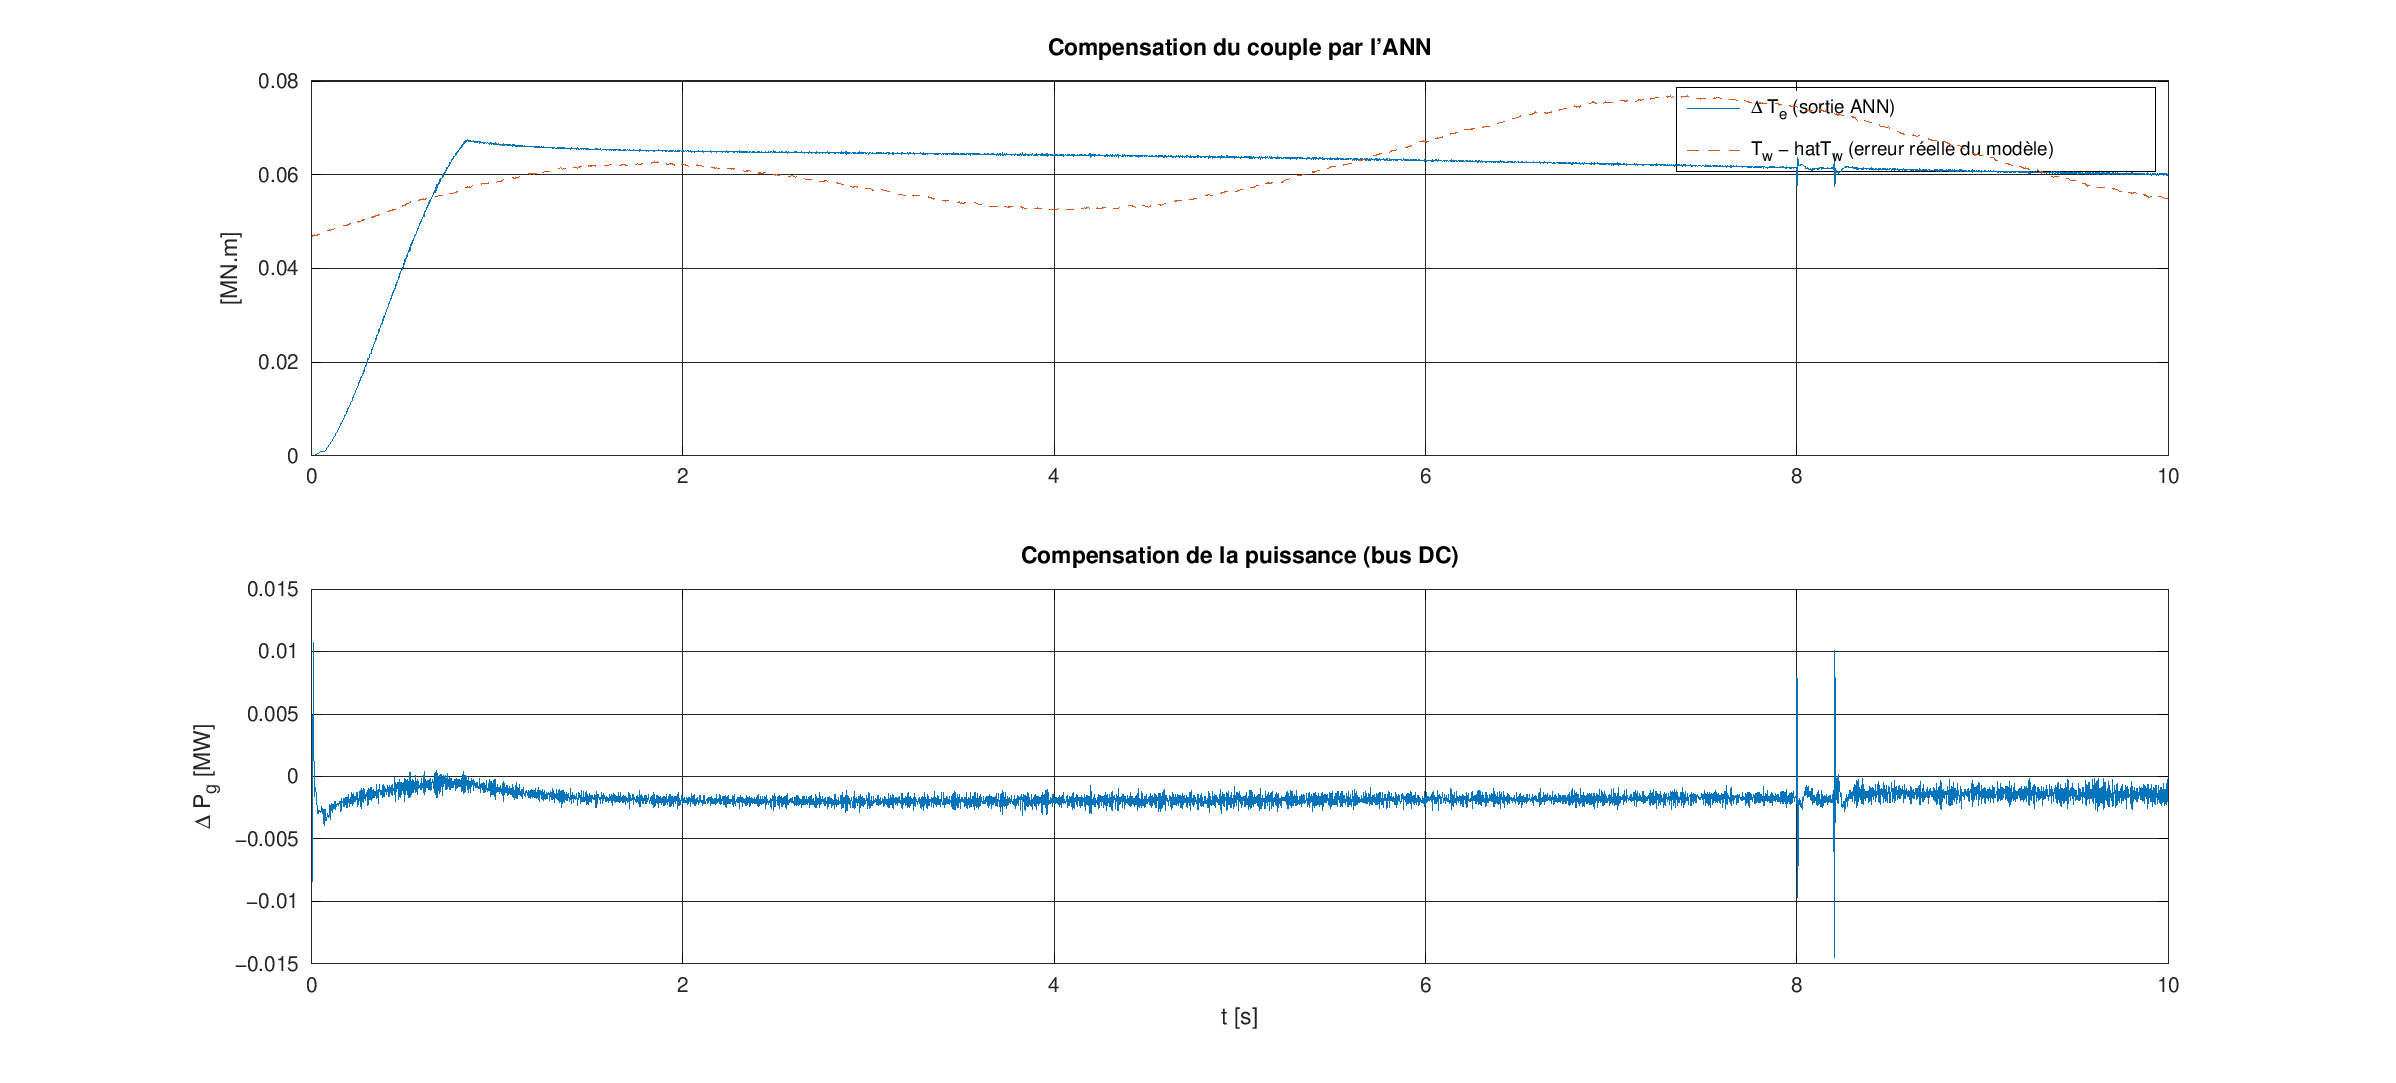
\includegraphics[width=0.95\textwidth]{fig_ann.png}
\caption{En haut : la sortie du réseau $\Delta T_e$ (bleu) et l'erreur réelle du modèle $T_w-\hat T_w$ (orange).}
\end{figure}
Dans le test de robustesse, le modèle sous-estime $T_w$ de 10\,\%, soit entre 0,05 et 0,077~MN$\cdot$m.
Le réseau \textbf{ne le sait pas}. Pourtant, en moins d'une seconde, $\Delta T_e \approx 0{,}065$~MN$\cdot$m,
c'est-à-dire à peu près la moyenne de l'erreur réelle. Il a « découvert » l'erreur uniquement à partir des
erreurs de vitesse. La partie qui varie lentement est corrigée par l'intégrale de la loi plate.

% =====================================================================
\section{La simulation : comment calcule l'ordinateur ?}
% =====================================================================

\paragraph{L'idée.} L'ordinateur ne peut pas résoudre les équations « d'un coup ». Il avance par très petits
pas ($T_s = 0{,}0001$~s) :
\[
x(t+T_s) \approx x(t) + T_s\cdot\frac{dx}{dt}
\]
« nouvelle valeur = ancienne + pas $\times$ vitesse de variation ». C'est la méthode d'Euler. Nous utilisons
une méthode plus précise (Runge-Kutta~4), qui calcule la vitesse de variation 4 fois dans le pas et en fait la moyenne.

\paragraph{Ce qui se passe à chaque pas (dans le script \texttt{PMSG\_Plate\_PBC\_ANN.m}).}
\begin{enumerate}
\item On lit le vent et la tension du réseau.
\item \textbf{(a)} MPPT : on calcule $\Omega^*$.
\item \textbf{(b)} Platitude, vitesse : on calcule $T_e^*$ puis $i_{sq}^*$.
\item \textbf{(c)} Passivité, redresseur : on calcule $\bv{v}_s^*$.
\item \textbf{(d)} Platitude, bus : on calcule $P_g^*$ puis $i_{gd}^*$.
\item \textbf{(e)} Passivité, onduleur : on calcule $\bv{v}_i^*$.
\item \textbf{(f)} Réseau de neurones : il apprend et calcule $\Delta T_e, \Delta P_g$ pour le pas suivant.
\item On applique les tensions au modèle et on avance d'un pas (RK4).
\end{enumerate}
On répète cela 100\,000 fois pour simuler 10 secondes.

% =====================================================================
\section{Lire les résultats}
% =====================================================================

\begin{figure}[h]
\centering
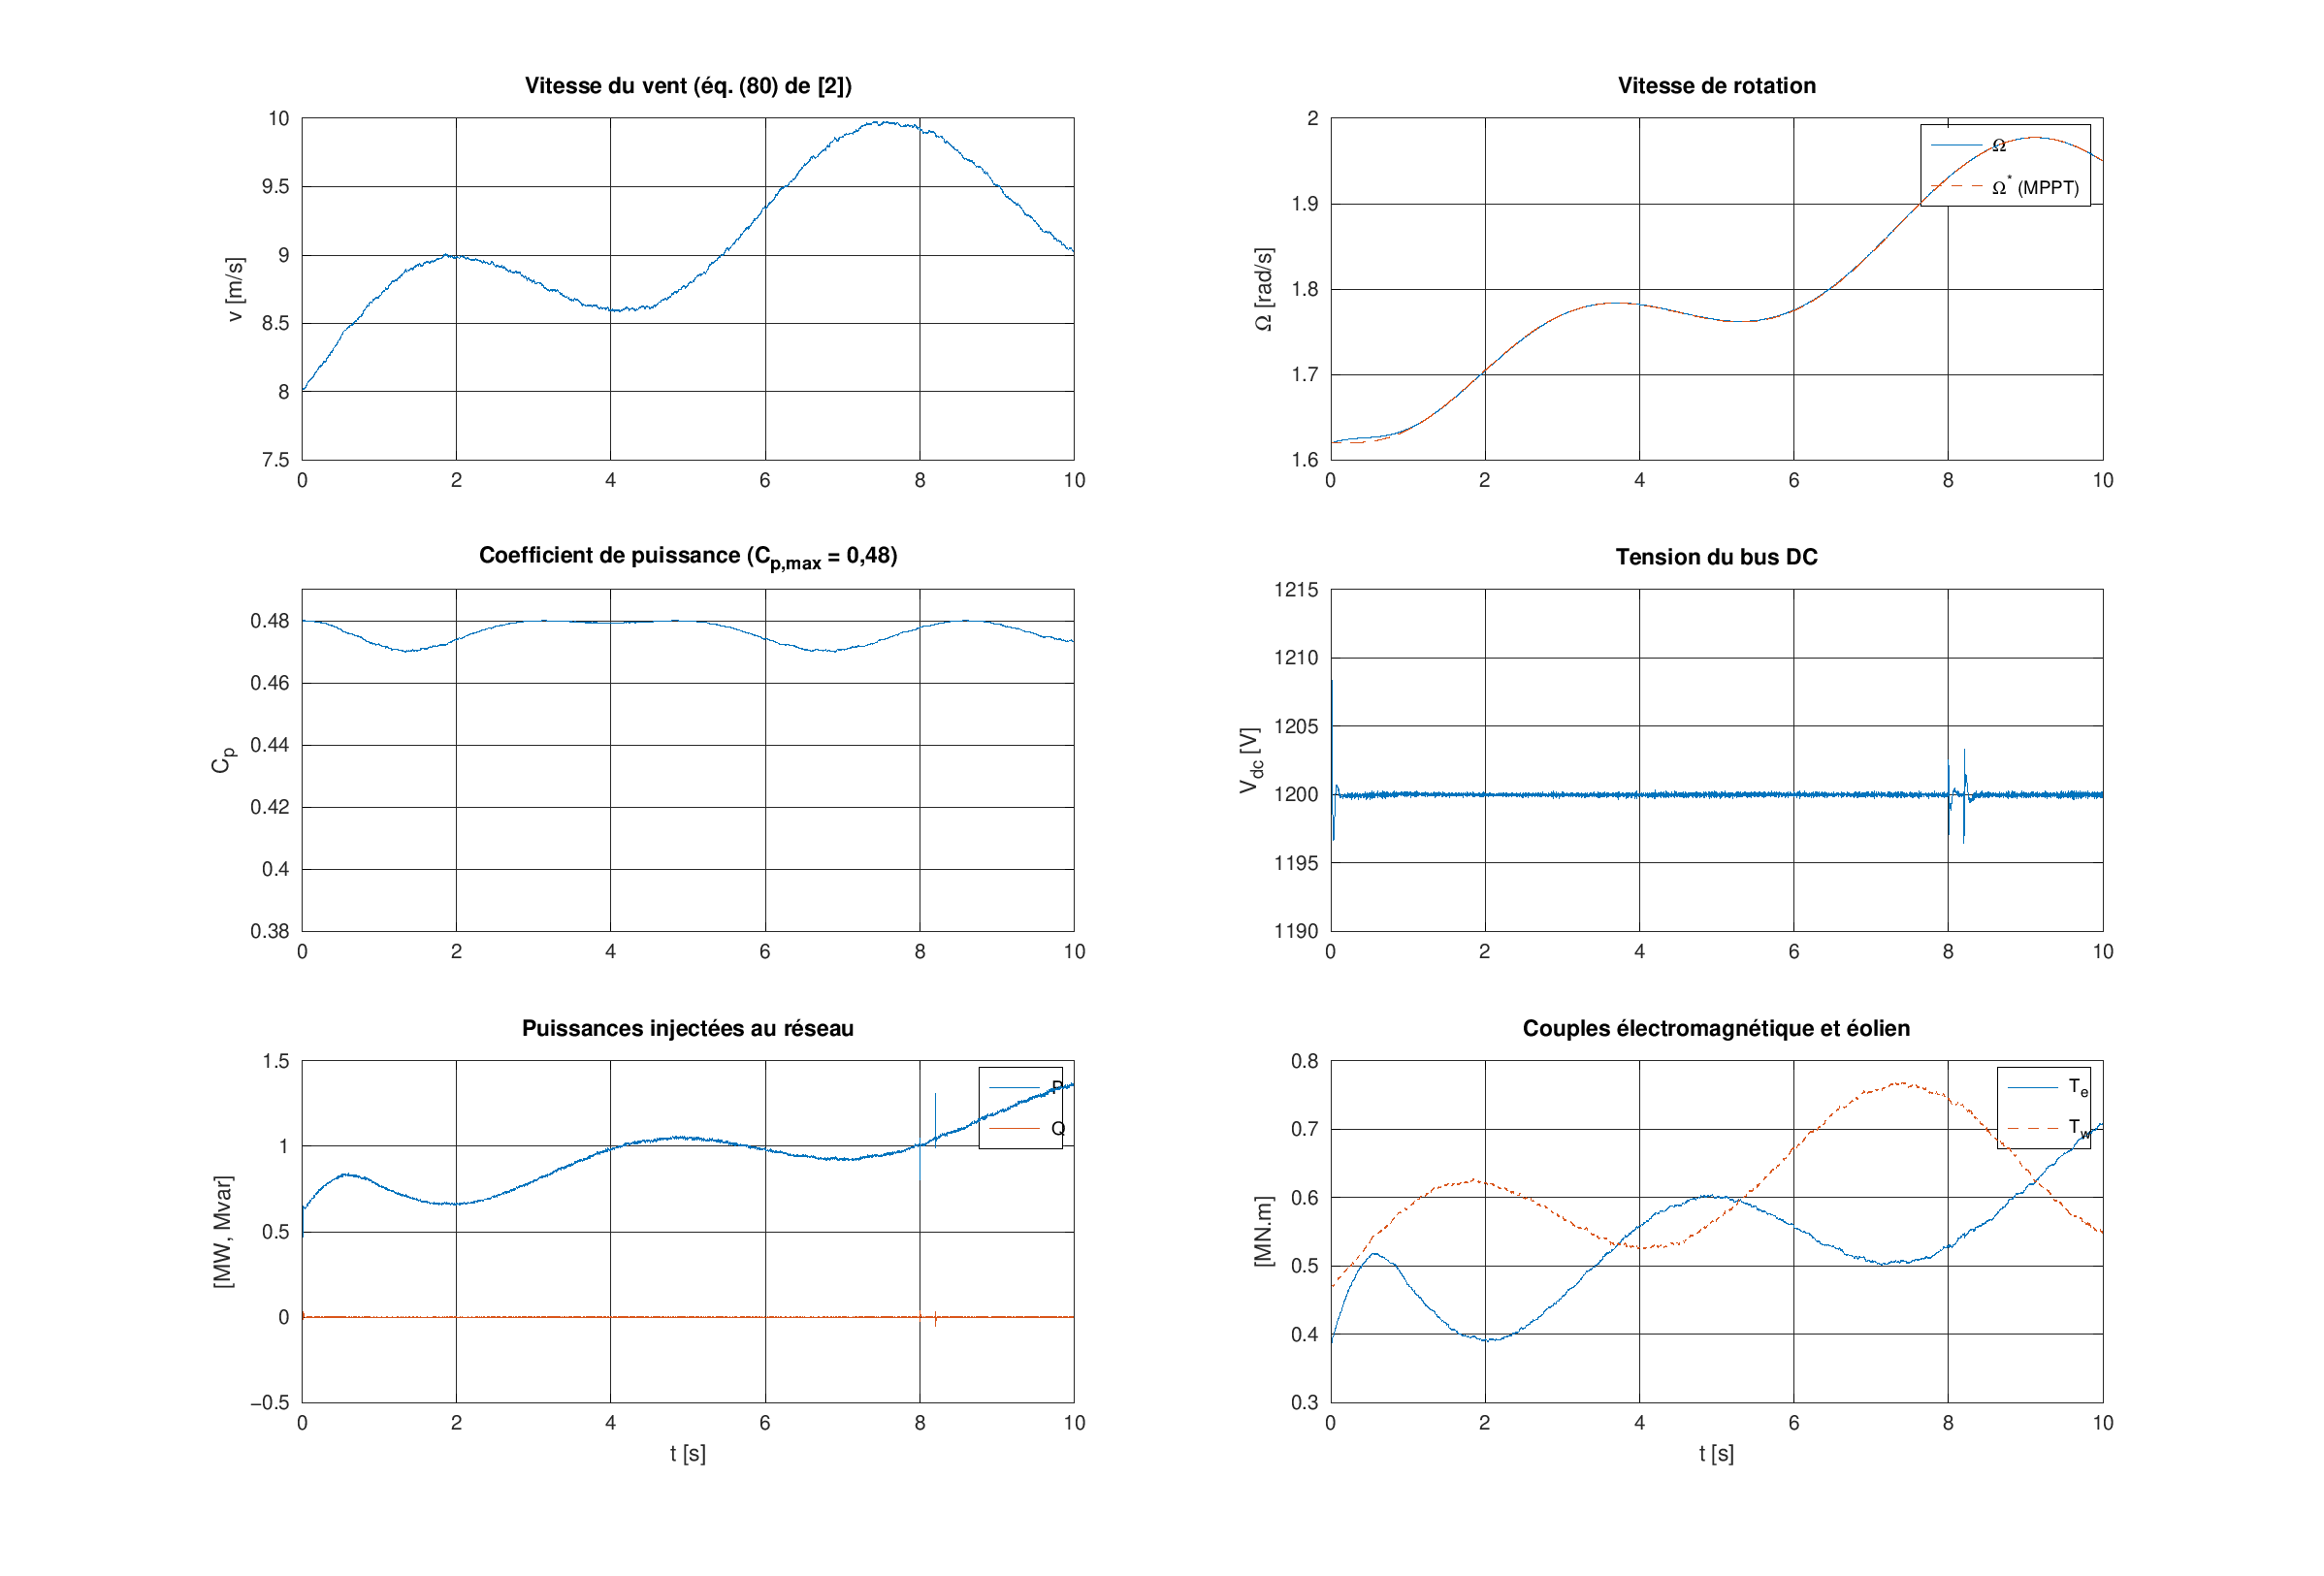
\includegraphics[width=\textwidth]{fig_ensemble.png}
\caption{Test de robustesse avec le réseau de neurones.}
\end{figure}
\begin{itemize}
\item \textbf{Le vent} (en haut à gauche) : le même vent que dans l'article.
\item \textbf{La vitesse} : $\Omega$ est exactement sur $\Omega^*$, la MPPT fonctionne.
\item \textbf{$C_p$} : entre 0,47 et 0,48, très proche du maximum.
\item \textbf{$V_{dc}$} : constant à 1200~V. À $t=8$~s, la tension du réseau baisse de 20\,\% (\textbf{creux de
tension}) : $V_{dc}$ bouge d'environ $\pm3{,}5$~V et revient en moins de 40~ms. Le plus grand écart
($10{,}4$~V) a lieu au démarrage, quand la commande part avec des paramètres faux.
\item \textbf{La puissance} : $P$ suit le vent et $Q = 0$.
\item \textbf{Les couples} : $T_e$ suit $T_w$ avec un retard, ce qui est normal à cause de l'inertie de la turbine.
\end{itemize}

\begin{center}
\begin{tabular}{lccc}
\toprule
Indicateur (test de robustesse) & sans ANN & avec ANN & amélioration\\
\midrule
Erreur de vitesse IAE & 0,0109 & 0,0067 & $-39\,\%$\\
Erreur du bus ISE & 1,30 & 1,16 & $-11\,\%$\\
Écart max de $V_{dc}$ (démarrage) & 10,4~V & 10,4~V & identique\\
Écart max de $V_{dc}$ (creux) & 3,35~V & 3,60~V & un peu plus grand\\
$C_p$ moyen & 0,476 & 0,476 & identique\\
\bottomrule
\end{tabular}
\end{center}
\textbf{IAE} = somme de la valeur absolue de l'erreur dans le temps. \textbf{ISE} = somme du carré de l'erreur.
Plus ils sont petits, meilleur est le suivi.

\begin{resume}
\Resume
Sans changer aucun coefficient de la commande de base, le réseau de neurones réduit l'erreur de vitesse de
39\,\% quand le modèle est faux. L'énergie produite ne change pas : l'amélioration porte sur la précision du
suivi, pas sur la quantité d'énergie.
\end{resume}

% =====================================================================
\section{Questions que l'encadrant peut poser (avec réponses)}
% =====================================================================

\begin{enumerate}
\item \textbf{Pourquoi une PMSG et pas une DFIG ?}
Parce qu'elle fonctionne sans multiplicateur (moins d'entretien), sans balais, avec un bon rendement.
En contrepartie, il faut un convertisseur dimensionné pour toute la puissance.

\item \textbf{Pourquoi $i_{sd}^* = 0$ ?}
Parce que le couple vient uniquement de $i_{sq}$ (machine à pôles lisses, $L_d=L_q$). Tout courant $i_{sd}$
crée des pertes inutiles.

\item \textbf{Pourquoi la platitude pour les boucles externes ?}
Parce que leurs équations sont simples et inversibles (arbre mécanique, bilan d'énergie). La platitude
utilise le modèle pour anticiper : elle est plus rapide qu'un PI qui attend l'erreur.

\item \textbf{Pourquoi l'énergie et pas la tension comme sortie plate du bus ?}
Parce que $\dot W = P_{msc} - P_{gsc}$ est linéaire en puissance, alors que l'équation de $V_{dc}$ est
non linéaire (elle contient $1/V_{dc}$).

\item \textbf{Pourquoi la passivité pour les courants ?}
Parce que les équations des courants ont une structure énergétique (couplage sans travail). La passivité
respecte cette structure et donne une preuve de stabilité simple ($dH/dt\le0$).

\item \textbf{Quelle différence entre notre réseau et un réseau « classique » ?}
Un réseau classique est entraîné à l'avance sur des données (hors ligne). Le nôtre apprend
\textbf{pendant le fonctionnement} (en ligne) : ses poids sont des variables qui évoluent avec le système.

\item \textbf{Pourquoi le réseau ajoute-t-il une correction au lieu de modifier les coefficients ?}
Pour que la commande de base, ses coefficients et sa preuve de stabilité restent inchangés. Le réseau
« aide » seulement : si on l'éteint, le système fonctionne avec la commande de base.

\item \textbf{Que signifie UUB ?}
L'erreur ne va pas forcément exactement à zéro, mais elle entre dans une petite zone autour de zéro et n'en sort plus.

\item \textbf{Les paramètres sont-ils réels ?}
Ceux de la machine, du bus et du réseau viennent d'un article publié (Hasan \& Shatil, AJSE 2021). Ceux de
la turbine viennent de l'encadrant. Seuls $J$, $B$ et $R_f$ sont des hypothèses.

\item \textbf{Quelles sont les limites du travail ?}
Pas de commande de l'angle de calage (vent inférieur au nominal), PLL idéale, résultats principaux avec le
modèle moyen, et la loi de vitesse utilise le vent mesuré.
\end{enumerate}

% =====================================================================
\section*{Annexe : lexique}
% =====================================================================
\begin{center}\small
\begin{tabular}{ll}
\toprule
Français & English\\
\midrule
machine synchrone à aimants permanents & permanent magnet synchronous generator (PMSG)\\
redresseur / onduleur & rectifier / inverter\\
MLI (modulation de largeur d'impulsion) & PWM\\
bus continu & DC link\\
coefficient de puissance $C_p$ & power coefficient\\
vitesse spécifique $\lambda$ & tip-speed ratio\\
recherche du point de puissance maximale (MPPT) & maximum power point tracking\\
commande par platitude & flatness-based control\\
sortie plate & flat output\\
commande passive (PBC) & passivity-based control\\
injection d'amortissement & damping injection\\
fonction de stockage / de Lyapunov & storage / Lyapunov function\\
réseau de neurones (ANN) & artificial neural network\\
poids / biais & weight / bias\\
couche cachée & hidden layer\\
rétropropagation & backpropagation\\
zone morte & dead-zone\\
uniformément ultimement borné (UUB) & uniformly ultimately bounded\\
creux de tension & voltage dip\\
\bottomrule
\end{tabular}
\end{center}

\end{document}
